% !TeX root = Tesis.tex
\documentclass[12pt, oneside, final, letterpaper, stu]{huthesis}

%%%% Paquetes %%%%%%%%%%%%%%%%%
\usepackage[utf8]{inputenc}
%\usepackage[latin1]{inputenc}
%\inputencoding{latin1}
%\usepackage[spanish]{babel}
\usepackage[T1]{fontenc}
%\usepackage[latin1]{inputenc}

%\usepackage[latin1]{inputenc}
%\usepackage[spanish]{babel}
\usepackage{graphicx}
\usepackage{xcolor,colortbl}
\usepackage{rotating}
\usepackage{times}
\usepackage{pdflscape}
\usepackage{graphicx}
\usepackage{amsmath}
\usepackage{amssymb}
\usepackage{amssymb}
\usepackage{amsmath}
\usepackage{mathrsfs}
\usepackage[spanish]{babel}
%\usepackage[print]{pdfscreen}
\usepackage{ae}
\usepackage{array}
\usepackage{textcomp}
\usepackage{amsmath}
\usepackage{amssymb}
\usepackage{subfig}
\usepackage{mathrsfs}
%\usepackage{matlab}
\usepackage{hyperref}
\usepackage{Portada}
%CORREGIR LA METODOLOGIA
\usepackage{placeins}

\usepackage{multirow}
\usepackage{fancyhdr}
\usepackage{algoritmo}
\usepackage{epsfig}
\usepackage{float}
% \usepackage{apacite}
\usepackage[style=apa, backend=biber]{biblatex}
\addbibresource{bibliografia.bib}

\usepackage{longtable}
\usepackage{rotating}


%%%%%%%%%%%
\usepackage{color}
\definecolor{gray97}{gray}{.97}
\definecolor{gray75}{gray}{.75}
\definecolor{gray45}{gray}{.45}

\usepackage{listings}
\lstset{ frame=Ltb,
framerule=0pt,
aboveskip=0.5cm,
framextopmargin=3pt,
framexbottommargin=3pt,
framexleftmargin=0.4cm,
framesep=0pt,
rulesep=.4pt,
backgroundcolor=\color{gray97},
rulesepcolor=\color{black},
%
stringstyle=\ttfamily,
showstringspaces = false,
basicstyle=\small\ttfamily,
commentstyle=\color{gray45},
keywordstyle=\bfseries,
% 
numbers=left,
numbersep=15pt,
numberstyle=\tiny,
numberfirstline = false,
breaklines=true,
}


\lstdefinestyle{consola}
{basicstyle=\scriptsize\bf\ttfamily,
backgroundcolor=\color{gray75},
}

\lstdefinestyle{C}
{language=C,
}
%%%%%%%%%%%


\usepackage{listings}
\usepackage{color}
\usepackage{multicol}

%\usepackage[latin1]{inputenc}
%\usepackage[utf8]{inputenc}

\hypersetup{backref=false, colorlinks=false}
\spanishdecimal{.}
\DeclareGraphicsExtensions{.pdf}
\def\tablesp{\def\baselinestretch{1.1}\large\normalsize}
\def\subtema{\subsubsection*}

\usepackage{enumitem,amssymb}
\newlist{todolist}{itemize}{2}
\setlist[todolist]{label=$\square$}

\usepackage{xcolor,colortbl}
\definecolor{verde}{rgb}{0,0.9,0}

%----------------------------------
% !TeX root = Tesis.tex
\hyphenation{  }
     % ---- Separaciones de palabras
\input{defmat}     % ---- Definiciones matemticas


%------------ Informacin de la Tesis
% \title{\LARGE {...}
% \title{ Desarrollo de un sistema web para el almacenamiento y representación de factores de riesgo cardiovascular en la Universidad de la Sierra Sur, empleando Bun y Node.js}	
\title{ Sistemas web para la gestión y evaluación del riesgo cardiovascular en una universidad usando Bun y Node.js
}	

\author{ Elietzer Jared Galicia Cordova }												%---> Autor
\usepackage[spanish]{babel}

\degreemonth{Enero}																		%---> Mes
\degreeyear{2026}																			%---> Ao
\degree{Licenciado en Informática}															%---> Grado
\institute{Instituto de Informática}														%---> Nombre del Instituto
\department{Instituto de Informática}														%---> Nombre del departamento
\university{Universidad de la Sierra Sur}													%---> Nombre universidad
\place{Miahuatlán de Porfirio Díaz Oaxaca, México.}											%---> Lugar
\advisor{M.T.I.E. Irving Ulises Hernández Miguel}{\ }	
%---> Directores
\titleen{SiBIB}
%\titleen{Sistema Para la Evaluacin Motriz de Miembros Superiores en Peditricos Empleando Guantes de Realidad Virtual.}  %---> Titutlo o subtitulo
%%%
%Algoritmo
\definecolor{dkgreen}{rgb}{0,0.6,0}
\definecolor{gray}{rgb}{0.5,0.5,0.5}
\definecolor{mauve}{rgb}{0.58,0,0.82}
\newlength\mylength
\newcolumntype{C}[1]{>{\centering\arraybackslash}p{#1}}
\setlength\mylength{\dimexpr\textwidth-5\arrayrulewidth-8\tabcolsep}

\lstset{frame=tb,
	language=C++,
	aboveskip=3mm,
	belowskip=3mm,
	numbers=left,
	showstringspaces=false,
	columns=flexible,
	basicstyle={\small\ttfamily},
	numberstyle=\tiny\color{gray},
	keywordstyle=\color{blue},
	commentstyle=\color{dkgreen},
	stringstyle=\color{mauve},
	breaklines=true,
	frame=leftline,
	breakatwhitespace=true
	tabsize=3
}
%%%%%%%%%%%%%%%%%%%%%%%%%%%%%%%%%%%%%%%%%%%%%%%%%%%%%%%%%%%%%%%%%%%%%%%%%%%%%555

\begin{document}
    \renewcommand{\tablename}{Tabla}
    \renewcommand{\listtablename}{Índice de tablas}  
    \maketitle
    \pagenumbering{arabic}
    \setcounter{page}{1}
    %\include{Presentacion}
    %\cleardoublepage
%   % !TeX root = Tesis.tex

\begin{resumen}

Uno de los desafíos en las áreas de computación e ingeniería es el desarrollo de sistemas, que permitan la automatización de los procesos que se generan durante la ejecución de pruebas experimentales, que requieren información bioeléctrica (estudios sobre emociones, memoria cognitiva, demencia, neuromarketing, por mencionar algunos). Además, el software representa un problema para los usuarios que utilizan de este tipo de sistemas, ya que generalmente para adquirirlo se requiere del pago de una licencia y en consecuencia se genera dependencia con el proveedor. El objetivo de este trabajo de investigación es diseñar, desarrollar y evaluar un sistema modular empleando software libre que permita obtener, almacenar, administrar y visualizar la información bioeléctrica obtenida de los sensores en tiempo real (un electroencefalógrafo, un sensor de ritmo cardíaco y un sensor de conductancia de la piel), información del expediente clínico electrónico, así como información adicional generada durante la ejecución de un experimento. Para la autenticación del sistema se cuenta con tres tipos de usuarios con privilegios específicos, así como dos niveles de seguridad, uno por medio de usuario y contraseña, y el otro por medio de una huella digital. Por otra parte, el sistema cuenta con la opción de exportar la información bioeléctrica de los experimentos en formato csv y reportes generales como el expediente clínico electrónico en formato pdf. El sistema que se presenta fue desarrollado empleando software libre basado en el modelo de procesos de ingeniería de la usabilidad y la accesibilidad para el diseño de interfaces, el modelo de proceso evolutivo para la mejora continua de prototipos y el Modelo-Vista-Controlador en la implementación de interfaces gráficas de usuario. Para la evaluación del sistema se realizaron dos tipos de pruebas, las pruebas de funcionalidad para validar los requerimientos y las pruebas de evaluación heurística para evaluar el nivel de usabilidad que presenta el sistema.
%Finalmente, se concluye que al desarrollar un sistema integrando diferentes tecnologías, empleando software libre y siguiendo un conjunto de metodologías, es posible obtener un sistema funcional y usable, para la automatización de la información en la ejecución de pruebas experimentales que requieren de información bioeléctrica.% que requieren de la información bioeléctrica.

\end{resumen}

\begin{abstract}

One of the challenges in the areas of computing and engineering is the development of systems that can modify the automation of the processes that can be performed during the execution of experimental tests that require bioelectrical information (studies on emotions, cognitive memory, dementia, neuromarketing, to mention some of them). Morover, for users who use this type-kind of system, it represents a problem, since in general, to purchase them, a license is required and, consequently, it is generated a dependence on the provider. The objective of this research work is to design, develop and evaluate a modular system using free software that allows obtaining, specifying, managing and visualizing the bioelectrical information obtaining the sensors in real time (an electroencephalograph, a heart rate sensor and a skin conductance), information from the electronic clinical record, as well as additional information generated during the execution of an experiment. For system authentication, there are three types of users with specific privileges and two levels of security, the first by using an username and password, and the other via fingerprint. The system has too the option of exporting the bioelectrical information of the experiments in csv format and general reports such as the electronic clinical record in pdf format. The system presented was developed using free software based on the usability and accessibility engineering process model for interface design, the evolutionary process model for continuous improvement of prototypes and the Model View Controller in the implementation of graphical user interfaces. For the evaluation of the system, two types of tests are used: the functionality tests to validate the requirements and the heuristic evaluation tests to evaluate the level of usability that the system presents. %Finally, it is concluded that by developing a system integrating different technologies, using free software and following a set of methodologies, it is possible to obtain a functional and usable system for the automation of information in the execution of experimental tests that requires biolectrical information.



%The automation of the processes that are carried out during the experimental tests that require the bioelectric information of an individual represents a challenge in the areas of computer science and engineering mainly, since it needs the integration and the configuration between the software (databases, controllers, communication networks, applications, among others) and hardware (sensors, information input and output devices, interaction devices, among others). In the market there are systems that have the objective but, they represent a problem when acquiring it for its high cost and also a dependency with the supplier is generated. The Bioelectric Information Based Information System (SIBIB) is a modular system, where the part of it allows obtaining, specifying and visualizing the bioelectric information of three sensors in real time produced by users during the interaction with a product or multimedia media. These are an electroencephalograph, a heart rate sensor and an electrical skin conductance sensor. Also, the system has two levels of security for access authentication, one by means of a username and password, and the other by means of a fingerprint. In comparison with other systems that carry out this process, it also allows the visualization of the information collected by the sensors in real time, its storage, the addition of comments and markers. There is also the option to export the information of the experiments and general reports such as the electronic clinical file. This system was developed using free software based on the usability and accessibility engineering process model for the design of its interfaces, the evolutionary process model for continuous prototype improvement and the controller view model for code implementation. of programming. For its evaluation two types of tests are used, the functionality tests and a heuristic evaluation, which is carried out by three evaluators. Finally, it is concluded that by generating a system integrating different technologies, a functional and usable system can be obtained for experimental tests that require bioelectric information.

%The realization of experimental tests to obtain bioelectrical information of an individual is a challenge for different investigations or projects, this is due to two factors that are necessary for the realization of these. The first one is the software and the second the hardware. In most cases you cannot use one without having access to the other. For this reason there are companies that focus on developing both the hardware for testing and the software for its use. The Information System Based on Bioelectric Information is a set of various technologies that deal with the collection, storage and visualization of real-time information produced by users during interaction with a product or multimedia media. The system consists of the integration of three sensors for the collection of bioelectric information. These are an electroencephalograph, a heart rate sensor and an electrical skin conductance sensor. The system also has two levels of authentication for access, one through a username and password, and the other through a fingerprint. Compared to other softwares that perform this process, this allows the visualization of the information collected by the sensors in real time, its storage, the addition of comments and bookmarks in files. There is also the option to export the information of the experiments and general reports such as the electronic clinical file. This system was developed based on the usability and accessibility engineering process model (MPIu + a).

%The Information System Based on Biometric Information is a set of various technologies that deal with the collection, storage and visualization of real-time information produced by biometric experiments. The system consists of the integration of three sensors for the collection of the bioelectrical information that a person produces during the interaction with some element, be it a product, a software or some multimedia element. The sensors integrated in the system are an electroencephalograph, a heart rate sensor and an electrical skin conductance sensor. The system has two levels of authentication for access, one through a username and password, and the other through a fingerprint. It allows the visualization of the information collected by the sensors in real time, its storage and the addition of comments and bookmarks in files. Also, there is the option to export the information of the experiments and general reports. This system was developed based on the usability and accessibility engineering process model.

\end{abstract}

\newpage
\thispagestyle{empty}

%\begin{publicaciones}

%\noindent Como parte de los resultados del trabajo de investigación
%desarrollado en esta tesis, se obtuvo el siguiente artículo (ejemplos para artículos resultado de tesis)s:

%\subsection*{Artículos en congresos internacionales}
%\subsubsection*{Aceptados}
%\begin{itemize}
%\item \textbf{González, L. A., Jarillo, A., Cruz, J.A., Gómez, V., García, A. M., y Domínguez O. A. (2012).}, \emph{Cartesian control
%application in haptic interfaces for motor rehabilitation purposes.}, IEEE ninth electronics (CERMA), Cuernavaca, Morelos, México.
%\end{itemize}
%\subsubsection*{Sometidos}
%\begin{itemize}
%\item \textbf{González, L. A., Jarillo, A., Cruz, J.A., Gómez, V., García, A. M., y Domínguez O. A. (2013).}, \emph{REyEMO a haptic system for rehabilitation purpuses.}, International Journal of Digital content Technology and its Applications (JDCTA), Korea.
%\end{itemize}

%\end{publicaciones}

 %    \cleardoublepage
    \newpage
    \tableofcontents
\clearpage
 %    \listoffigures
  % \cleardoublepage
   %\listoftables
%   \cleardoublepage
    \pagenumbering{arabic}
    

% TESISSS
% !TeX root = Tesis.tex

%\setlength{\parskip}{-1cm}%
%\chapter{Anteproyecto}


\section{Antecedentes} 
Los sistemas  de monitorización remota han evolucionado durante los últimos años incrementando su autonomía, portabilidad y funcionalidad. Por otra parte, el avance en el diseño de biosensores y la generación de algoritmos en la adquisición y procesamiento de bioseñales, han permitido incrementar las áreas de oportunidad en el campo de la investigación. Por ejemplo, en el área de la psicología para la evaluación y experimentación de las emociones, la carga cognitiva y los estados mentales, con el fin de extraer  información para su estudio y análisis.

El término bioseñal se aplica a todos los tipos de señales fisiológicas que pueden ser medidas y controladas, entre las más conocidas se tienen  las generadas por el cerebro (Electroencefalograma (EEG)), la respuesta galvánica de la piel (por sus siglas en inglés GSR) y la Frecuencia Cardíaca (FC). El tratado de bioseñales ha permitido su aplicación en diversos campos de estudio en el área tecnológica, como en la Interacción Humano Computadora (IHC).  En este caso, a partir de la identificación del nivel de carga cognitiva es posible evaluar patrones de comportamiento durante la interacción entre un usuario y un producto tecnológico. Algunos ejemplos de estos productos pueden ser: una pantalla táctil, teléfonos móviles, tabletas, sitio web, aplicaciones móviles y de escritorio entre otros.

 A lo largo de las últimas décadas, la adquisición y monitoreo de bioseñales  han tenido importantes avances tecnológicos. \cite{avalos}, en su tesis de maestría propone un marco de trabajo (framework) enfocado en el tratamiento de bioseñales. En este caso se estudió una  electrocardiografía obtenida a través de dispositivos corporales inteligentes. La integración de bioseñales busca servir de apoyo para el análisis y entendimiento de los patrones de un usuario en actividades académicas,  como el diseño de gramáticas libres de contexto. A través de esta propuesta se demostró la funcionalidad para la adquisición e integración de una sola bioseñal (EEG), sin embargo, no se establece si el sistema es capaz de integrar más de una de ellas.
 
La detección de carga cognitiva es beneficiosa en varias aplicaciones de la IHC, incluida la gestión de la atención y la adaptación de la interfaz de usuario. Sin embargo, la investigación actual sobre la detección de carga cognitiva basada en bioseñales precisas y en tiempo real carece de comprensión de la longitud de ventana óptima y mínima en la segmentación de datos. \cite{tervone}, presentan un análisis comparativo de longitudes de ventana ultracortas (30s o menos) en la detección de carga cognitiva con un dispositivo portátil. Las funciones de frecuencia cardíaca, variabilidad de la frecuencia cardíaca, respuesta galvánica de la piel y temperatura de la piel se extraen en seis longitudes de ventana diferentes y se utilizan para entrenar un clasificador de aumento de gradiente extremo para detectar la carga cognitiva y el descanso. Este análisis proporciona una base prometedora para futuras aplicaciones en tiempo real con sensores portátiles.

La tecnología se encuentra inmersa en nuestra vida diaria, cuando nos imaginamos el futuro, siempre lo hacemos con la certeza de que existirán nuevas tecnologías y formas de comunicarnos. \cite{vaquero}, propone el desarrollo de aplicaciones e interfaces de Realidad Virtual (RV) capaces de adaptarse al estado cognitivo y emocional del cerebro humano, lo cual involucra la medición y la detección de patrones en la actividad cerebral al analizar los datos medidos mediante bioseñales de tipo EEG. Asimismo  \cite{vaquero}, estudia la posibilidad de integrar en un sistema como el descrito un modo de reconocer en tiempo real patrones de actividad cerebral asociados a distintos estados emocionales y cognitivos, como el estrés, la imaginación motora y la carga cognitiva. Todo ello con el fin de alterar el entorno virtual para adaptarse a estas nuevas circunstancias. Una de las desventajas es que al igual que \cite{avalos}, solo emplean el estudio de una bioseñal.

En la IHC para determinar si un producto cumple con los requerimientos de usabilidad se debe evaluar la eficiencia, la eficacia y la satisfacción. Para ello tradicionalmente se emplean técnicas subjetivas, que muchas veces los resultados varían dependiendo del estado emocional del sujeto. Actualmente, se están estudiando aplicar técnicas objetivas, donde el manejo de bioseñales juega un papel importante. El desarrollo de un software para la obtención de un conjunto de bioseñales a partir de dispositivos inteligentes, sería una excelente aportación para investigadores en cualquier campo de estudio, que estén interesados en realizar un análisis con la información obtenida. Este tipo de software ya existe en el mercado, pero muchas veces no es accesible debido a las exigencias del equipo computacional del investigador. Otra desventaja es que la mayoría de los sistemas existentes no son de código abierto, estos se conectan a los servidores de empresas que brindan servicios en la nube, las cuales muchas veces en sus políticas no establecen la privacidad de los datos.
|

\section{Planteamiento del problema} 
La pregunta de investigación es la siguiente: ¿Cómo desarrollar un sistema diseñado mediante un framework UX y de software libre, que  proporcione el nivel de carga cognitiva a partir del tratamiento de bioseñales como parte de la evaluación en el  ciclo de vida del Diseño Centrado en el Usuario (DCU)?


\section{Justificación}
Durante el desarrollo de un sistema se deben establecer las metodologías que se van emplear, por un lado la Ingenería de Software(IS) considera metodologías centradas en la funcionalidad del sistema, mientras que en el Diseño Centrado en el Usuario (DCU) su objetivo se basa en la experiencia del usuario. Con respecto a las metodologías de la IS una de las ventajas del DCU es que involucra al usuario en todas las etapas de su ciclo de vida. Para determinar la usabilidad de un sistema o software existen diversas técnicas, que permiten medir el nivel de usabilidad a partir de la experiencia del usuario durante la interacción.

Una de las etapas más importantes del DCU es la etapa de evaluación, ya que en esta se determina el nivel de usabilidad que presenta el sistema antes de su lanzamiento. En ella se aplican  métodos tradicionales como indagación, inspección y test, los cuales se basan en examinar las interfaces y su interacción con el usuario, además establecen métricas para cuantificar el rendimiento, la satsifacción y la eficacia del usuario con el sistema. Durante la interacción entre un usuario y un sistema, en el usuario se generan emociones y estados cognitivos, además cuando un usuario intenta resolver una tarea en específico es posible que experimente diferentes niveles de carga cognitiva. Los métodos tradicionales ya mencionados no evalúan el nivel de carga cognitiva durante la interacción de manera objetiva. Hoy en día gracias al avance tecnológico es posible determinar el nivel de carga cognitiva a través del estudio de las señales fisiológicas.

En la actualidad existen dispositivos fisiológicos que nos permiten controlar  y evaluar patrones de comportamiento, carga cognitiva y emociones mediante la adquisición de bioseñales. En la IHC la obtención de este tipo de señales permite conocer y analizar patrones de comportamiento de las personas al interactuar con un sistema informático, con el fin de desarrollar software centrado en las necesidades y características de los usuarios. 

La detección de carga cognitiva basada en bioseñales en tiempo real carece de herramientas tecnológicas accesibles y usables, que nos permitan el tratamiento de bioseñales para su estudio y análisis. El desarrollo de un software libre, que permita el tratamiento de bioseñales y diseñado mediante un framework UX (basado en la experiencia de usuario) serviría como un sistema de apoyo durante el proceso de evaluación. Los beneficiarios con este sistema serían ingenieros de pruebas, investigadores y evaluadores de usabilidad, que deseen complementar las evaluaciones de experiencia de usuario con una evaluación del estado cognitivo en tiempo real. 




%\section{Hipótesis}
%A continuación se presentan las hipótesis que se planean probar al concluir esta investigación.

%\subsection*{Hipótesis general}


%\subsection*{Hipótesis específicas}


\section{Objetivos}
\subsection{Objetivo general}
Desarrollo de un sistema diseñado mediante un framework UX y de software libre, que  proporcione el nivel de carga cognitiva a partir del tratamiento de bioseñales como parte de la evaluación en el  ciclo de vida del Diseño Centrado en el Usuario (DCU.


\subsection{Objetivos específicos}

\begin{itemize}
	\item Determinar y aplicar las técnicas de evaluación de usabilidad y de análisis en el diseño centrado en el usuario.
	\item 
	Conocer sobre la teoría de la carga cognitiva, la medición de las emociones, las señales psicofisiológicas.
	\item Determinar si los sensores psicofisiológicos son capaces de discernir realmente los estados cognitivos y emocionales en cada etapa de evaluación de DCU.
	\item Aplicar o diseñar algoritmos de procesamiento de bioseñales
	\item Diseñar un plan de pruebas de usabilidad.
\end{itemize}
\clearpage

\section{Metodología}

Los pasos que se llevarán  a cabo para el desarrollo de esta investigación son los siguientes:
\begin{itemize}

 \item \textbf{Búsqueda bibliográfica:} Búsqueda de documentación con base en las tecnologías y dispositivos que se desean integrar en este sistema. 


\item \textbf{Diseño:} El diseño se realizará en base a la metodología Design Thinking dividida en cinco fases: empatizar, definir, idear, prototipar y evaluar. Esta metodología consiste en un proceso iterativo entre los diferentes fases con el fin de generar soluciones basadas en las necesidades reales de los usuarios. 

\item \textbf{Desarrollo:} En esta etapa se buscará implementar una metodología que considere la Ingeniería de Software y la usabilidad.

		
\item \textbf{Redacción y revisión:} La redacción se llevará a cabo conforme el producto se vaya desarrollando.

\item \textbf{Evaluación del sistema:} En esta etapa se evaluará el sistema mediante la técnicas de evaluación de la usabilidad: indagación, inspección y test.
\section{Cronograma}
\begin{figure}[htb]
	\centering
	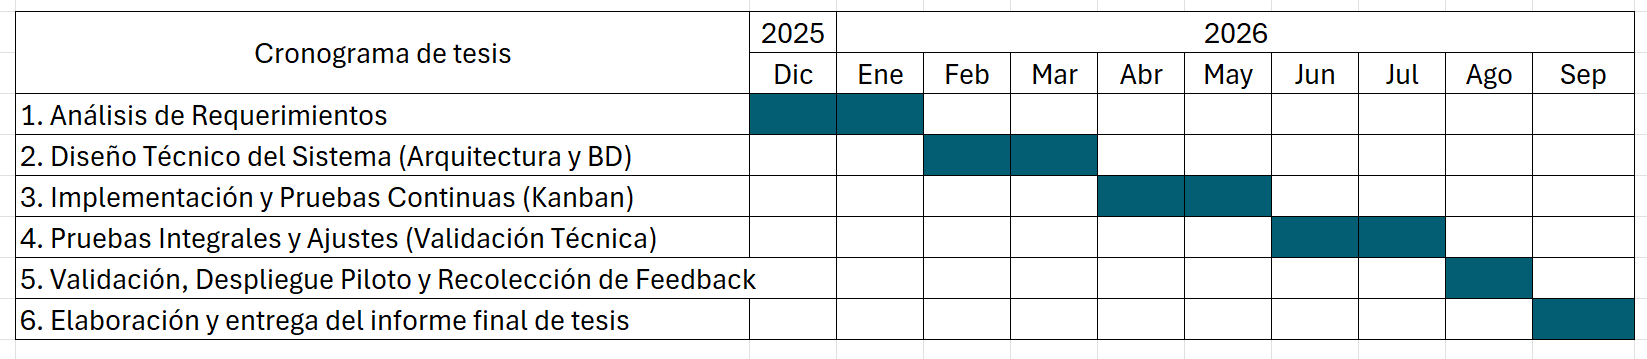
\includegraphics[width=\textwidth]{imagenes//cronograma.jpg}
	\caption{Cronograma del proyecto}\label{f:fig1y2}
	Fuente: Elaboración propia
\end{figure}
%\end{itemize}

%\section{Organización de la Tesis}
%A continuación se describe la organización de la tesis.

%\begin{itemize}
%	\item Capítulo 1: ``Introducción'', se incluyen los antecedentes del proyecto, el planteamiento del problema, la justificación, los objetivos y fundamentos del proyecto de investigación.
%	\item Capítulo 2: ``Análisis de fundamentos'', se incluyen los conocimientos fundamentales sobre los cuales se encuentra basado el proyecto, así también, los principios básicos para el entendimiento del trabajo.
%	\item Capítulo 3: ``Diseño de la arquitectura del sistema'', se presenta la integración de una arquitectura basada en el diseño centrado en el usuario y una metodología ágil en el desarrollo. Se exponen los procesos o técnicas que se emplearon para diseñar el sistema considerando las necesidades del usuario.
%	\item Capítulo 4: ``Desarrollo de la arquitectura del sistema'', se define la codificación, la descripción de los datos, diseño e implementación de las pruebas.
%	\item Capítulo 5: ``Pruebas y evaluación del sistema'', se presentan las pruebas realizadas al sistema y los resultados obtenidos de estas. Las pruebas diseñadas se evalúan con el apoyo de tres evaluadores.
%	\item Capítulo 6: ``Conclusiones y trabajos a futuro'', contiene las conclusiones y los trabajos a futuro de este proyecto de investigación.
\end{itemize}

%\clearpage
%\section{Cronograma}
%A continuación se presenta el cronograma de tiempo que se planea implementar para elaborar el proyecto de investigación:

%\begin{figure}[htb]
%	\centering
%	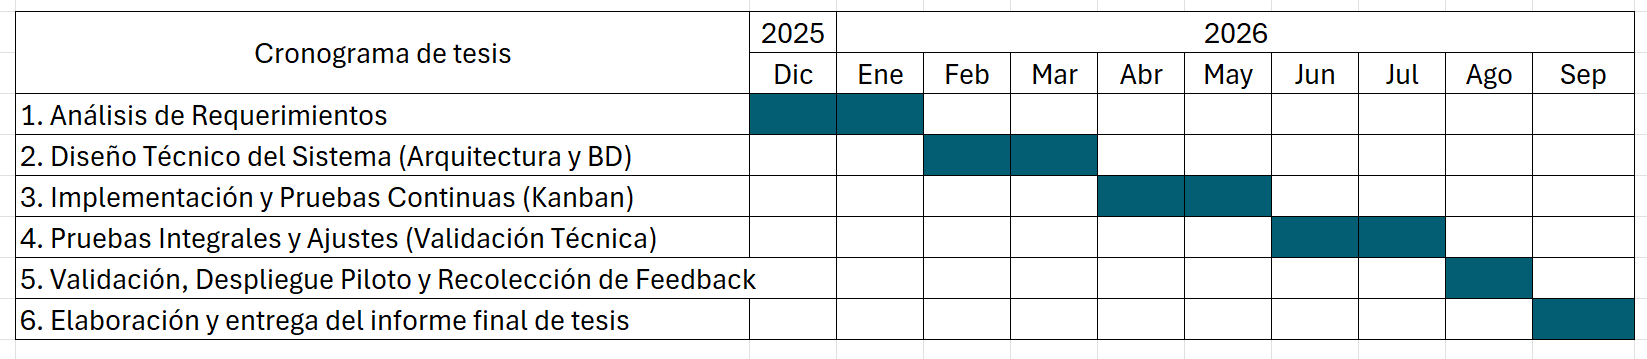
\includegraphics[width=\textwidth]{imagenes//cronograma.png}
%	\caption{Cronograma}\label{f:fig1y2}
%	Fuente: Elaboración propia
%\end{figure}

%\section{Índice tentativo}
%\begin{description}
%	\item[Capítulo 1.] Introducción
%		\begin{description}
%			\item 1.1. Antecedentes
%			\item 1.2. Planteamiento del problema
%			\item 1.3. Justificación
%			\item 1.4. Hipótesis
%			\item 1.5. Objetivos
%			\item 1.6. Organización de la tesis		
%		\end{description}
%	\item[Capítulo 2.] Análisis de fundamentos
%		\begin{description}
%			\item 2.1. Introducción
%			\item 2.2. Batería Neuropsicológica de Funciones Ejecutivas y Lóbulos Frontales 2 (BANFE-2)
%				\begin{description}
%					\item 2.2.1. Batería neuropsicológica
%					\item 2.2.2. Funciones ejecutivas
%					\item 2.2.3. Lóbulos frontales
%					\item 2.2.4. Evaluación neuropsicológica
%					\item 2.2.5. Prueba neuropsicológica
%					\item 2.2.6. Pruebas de la BANFE-2
%					\item 2.2.7. Expediente Clínico Electrónico (ECE)		
%				\end{description}			
%			\item 2.3. Búsqueda de sistemas informáticos para la BANFE-2
%				\begin{description}
%					\item 2.3.1. Sistemas comerciales
%					\item 2.3.2. Sistemas propietarios
%					\item 2.3.3. Sistemas gratuitos		
%				\end{description}
%			\item 2.4. Diseño centrado en el usuario
%				\begin{description}
%					\item 2.4.1. Principios del DCU
%					\item 2.4.2. Proceso de DCU
%				\end{description}		
%			\item 2.5. Metodologías de Ingeniería de Usabilidad
%				\begin{description}
%					\item 2.5.1. Ingeniería de Usabilidad
%					\item 2.5.2. Tipos de metodologías
%				\end{description}
%			\item 2.6. Metodologías de Ingeniería de Software
%				\begin{description}
%					\item 2.6.1. Ingeniería de Software
%					\item 2.6.2. Metodologías clásicas
%					\item 2.6.3. Metodologías evolutivas
%					\item 2.6.4. Metodologías ágiles
%				\end{description}
%			\item 2.7. Estándares relacionados con el DCU
%				\begin{description}
%					\item 2.7.1. INTE/ISO/IEC 9241-210. Diseño centrado en la persona para sistemas interactivos
%					\item 2.7.2. INTE/ISO 9241-151. Directrices para las interfaces de usuario Web
%				\item 2.7.3. INTE/ISO 9241-171. Guías sobre accesibilidad del software
%					\item 2.7.4. INTE/ISO 9241-125. Guía relativa a la presentación visual de la 	información	
%				\end{description}	
%			\item 2.8. Tecnologías de desarrollo		
%			\item 2.9. Patrones de arquitectura						
%			\item 2.10. Conclusión			
%		\end{description}		
%	\item[Capítulo 3.] Diseño de la arquitectura de la aplicación web
%		\begin{description}
%			\item 3.1. Introducción
%			\item 3.2. Metodología Scrum
%			\begin{description}
%				\item 3.2.1. Metodología ágil
%$				\item 3.2.2. Funcionamiento de Scrum
%		\end{description}
%			\item 3.3. Modelo de proceso de Ingeniería de la Usabilidad y accesibilidad (MPIu+a)
%			\begin{description}
%				\item 3.3.1. Características del modelo
%				\item 3.3.2. Etapas del modelo
%			\end{description}
%			\item 3.4. MPIu+a ágil: Una metodología pensada en el usuario
%			\begin{description}
%				\item 3.4.1. Introducción
%				\item 3.4.2. Diferencias entre Scrum y MPIU+a
%				\item 3.4.3. Beneficios de la integración de Scrum con DCU
%				\item 3.4.4. Integración de MPIu+a con Scrum
%			\end{description}		
%			\item 3.5. Tecnologías implementadas
%			\item 3.6. Conclusión			
%		\end{description}		
%	\item[Capítulo 4.] Desarrollo de la aplicación web
%		\begin{description}
%			\item 4.1. Introducción
%			\item 4.2. Descripción de los módulos del sistema
%			\item 4.3. Diseño de las pruebas del sistema
%			\item 4.4. Conclusión
%		\end{description}	
%	\item[Capítulo 5.] Pruebas y evaluación de la aplicación web
%		\begin{description}
%			\item 5.1. Introducción
%			\item 5.2. Pruebas funcionales o de caja negra	
%			\item 5.3. Evaluación heurística
%			\item 5.4. Pruebas de usabilidad
%			\item 5.5. Conclusión
%		\end{description}		
%	\item[Capítulo 6.] Conclusiones y trabajos a futuro
%	\item[Referencias] 						
%\end{description}



\section{Marco técnico y conceptual}
    \section{Introducción}
    \subsection{Sistemas de información en el ámbito de la salud}
    \subsection{Riesgo cardiovascular}
    \subsubsection{Factores de riesgo cardiovascular}
    \subsubsection{Clasificación del riesgo cardiovascular}
    \subsection{Sistemas web}
    \subsubsection{Arquitectura de sistemas web}
    \subsubsection{Aplicaciones web modernas}
    \subsection{Tecnologías utilizadas}
    \subsubsection{Bun}
    \subsubsection{Node.js}
    \subsubsection{Frameworks y librerías empleadas}
    \subsubsection{Base de datos}
    \subsection{Usabilidad}
    \subsubsection{Concepto de usabilidad}
    \subsubsection{Principios de usabilidad}
    \subsubsection{Usabilidad en sistemas web de salud}
    \subsection{Seguridad de la información}
    \subsubsection{Protección de datos personales}
    \subsubsection{Buenas prácticas de seguridad en sistemas web}
    
    \subsection{Trabajos relacionados}
 % %%%%%%%%%%%%%%%%%%%%%%%%%%%%%%%%%%%%%%%%%%%%%%%%%%%%%%%%%%%%%%%
    \section{Capítulo III: Diseño y desarrollo del sistema}
    
    \subsection{Introducción}
    \subsection{Análisis de requisitos}
    \subsection{Prototipado de baja fidelidad}
    \subsection{Pruebas de prototipado}
    \subsection{Prototipado de AF}
    \subsection{Pruebas de usuario}
    \subsection{Resultados}
    \subsection{Conclusiones}
% %%%%%%%%%%%%%%%%%%%%%%%%%%%%%%%%%%%%%%%%%
    \section{Capítulo IV: Resultados}
    \subsection{Introducción}
    \subsection{Resultados del desarrollo del sistema}
    \subsection{Resultados de las pruebas}
    \subsection{Evaluación del sistema}
    \subsection{Conclusiones}
% %%%%%%%%%%%%%%%%%%%%%%%%%%%%%%%%%%%%%%%%%%%%%%%%%%%%%%%%%
    \section{Capítulo V: Conclusiones y trabajos futuros}
    \subsection{Conclusiones}
    \subsection{Limitaciones del estudio}
    \subsection{Trabajos futuros}
% \endgroup

	% \bibliography{bibliografia}
 %        \cite{rengel2024efectos}
 %        \cite{tervone}
	% \bibliographystyle{apacite}
\printbibliography
\end{document}
